\section{A JSON Validation and XML/JSON Translation Web Service}

To demonstrate our OpenMath-JSON encoding, we have created a web site which can be found
at~\cite{openmathjson:web}.  This site is implemented in TypeScript and encapsulated using
docker~\cite{docker:webpage} container. It serves three purposes:

Primarily, it serves as a presentation of the encoding, providing examples and documenting it's usage. 

\begin{figure}\centering
  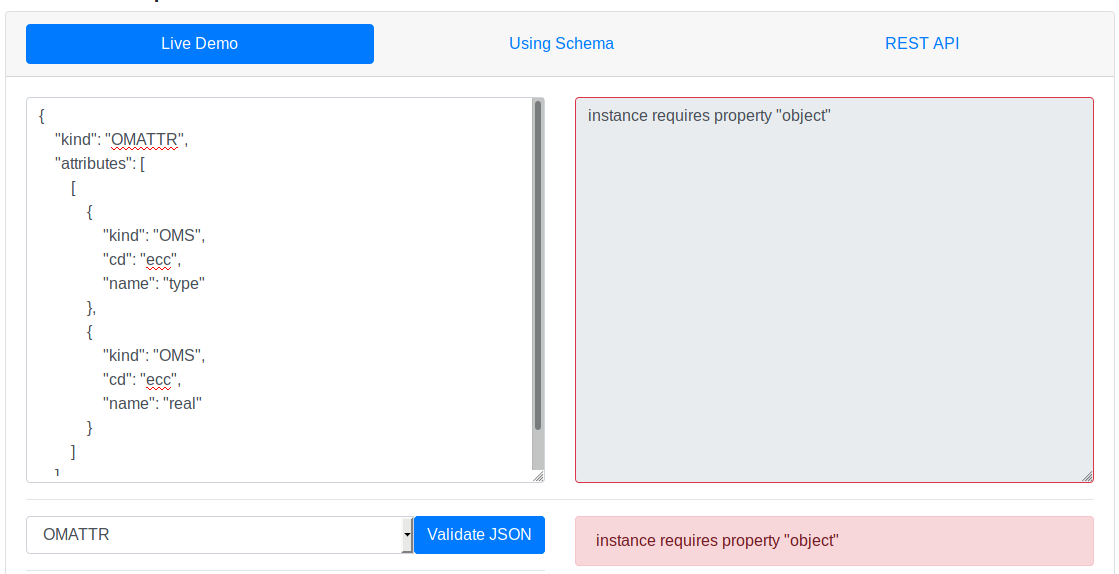
\includegraphics[width=\textwidth]{images/validate}
  \caption{Interface for validating an OpenMath object. }\label{figure:validate}
\end{figure}

Secondly, it enables validation of OpenMath JSON objects. This can be seen in Figure~\ref{figure:validate}.
The user can enter some JSON, press the \textit{Validate JSON} button, and receive immediate feedback if their JSON is a valid OpenMath object or not. 
In particular, the user can also see a detailed error message if their object is not valid OpenMath JSON. 

This makes use of the OpenMath JSON schema, and validates the users' JSON using a generic JSON Schema Validator. 
Furthermore, this is also exposed using a REST API, enabling easy validation of OpenMath JSON in other applications. 

\begin{figure}\centering
  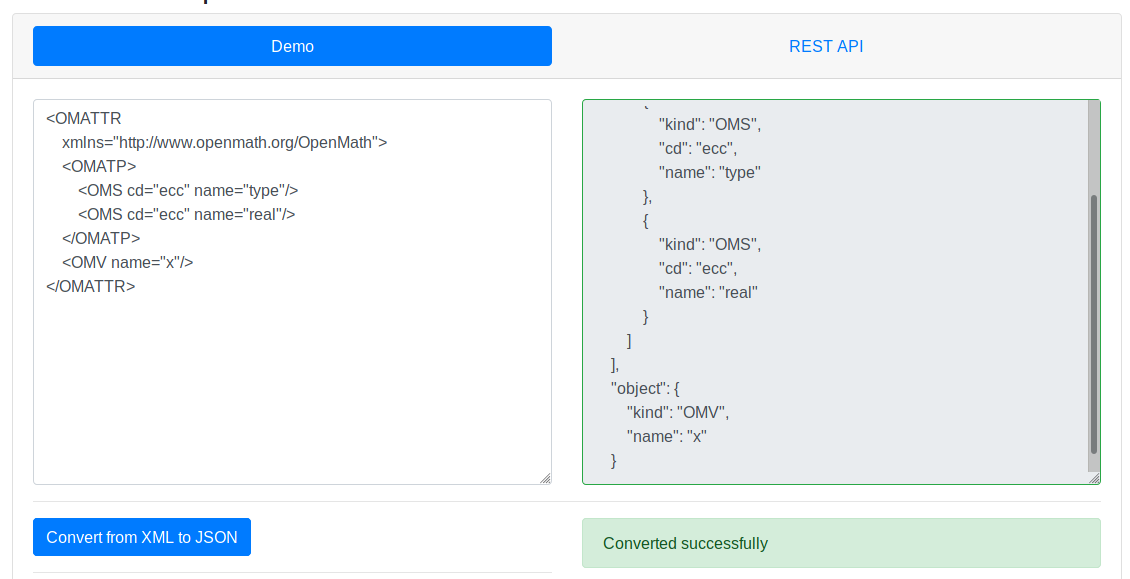
\includegraphics[width=\textwidth]{images/xml2json}
  \caption{Interface for converting OpenMath XML to JSON.}\label{figure:xml2json}
\end{figure}

\begin{figure}\centering
  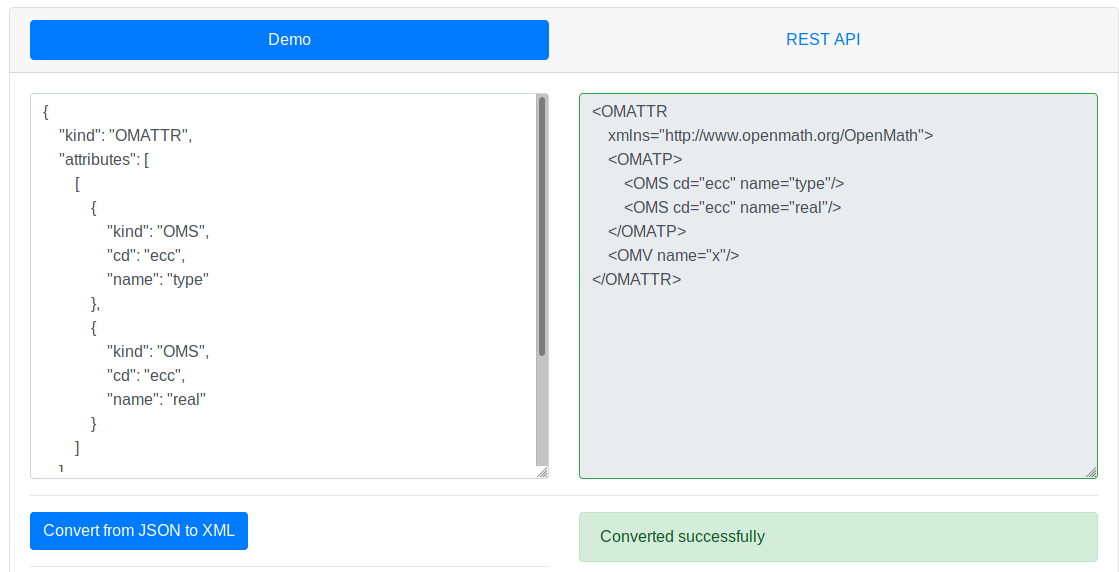
\includegraphics[width=\textwidth]{images/json2xml}
  \caption{Interface for converting OpenMath JSON to XML.}\label{figure:json2xml}
\end{figure}

Finally, it translates between XML and JSON encoded OpenMath objects. as for validation,
the site enables the user to enter some JSON and be presented with some XML and
vice-versa; see Figures~\ref{figure:xml2json} and \ref{figure:json2xml}.

As we designed our encoding with this translatability goal in mind, the implementation of
it was straight-forward.  For programmatic access, translation and validation are also
exposed using a REST API.

%%% Local Variables:
%%% mode: latex
%%% TeX-master: "paper"
%%% End:


%  LocalWords:  openmathjson:web centering includegraphics textwidth textit xml2json
%  LocalWords:  json2xml
